% ============================ Enrico Ribiani 16-03-2021 ====================================================================
% Base per i documenti  
\documentclass[12pt]{article}
% ------------ pacchetti necessari ----------------
\usepackage[a4paper, total={6in, 8in},margin=1in]{geometry} % formattazione decente della pagina
\usepackage{graphicx}                            % need for figure
\usepackage{amsmath}
\usepackage{amsfonts}                            % if you want the fonts
\usepackage{amssymb}                             % if you want extra symbols
\usepackage{graphicx}  
\renewcommand{\figurename}{Figura}  
\renewcommand{\contentsname}{Indice}                        % need for figures
\usepackage{mathptmx}
\usepackage{float}                               % serve per mettere tabelle e immagini dove si vuole 
\usepackage[utf8]{inputenc}
\usepackage{textcomp}
\usepackage[hang,flushmargin,bottom]{footmisc}   % footnote format
\usepackage{fancyhdr, lastpage}
\usepackage{titlesec}
\usepackage[table,dvipsnames]{xcolor}
%\pagestyle{fancy}
%\renewcommand{\headrulewidth}{0pt}
%\renewcommand*\contentsname{Indice}
\titleformat{\section}{\normalsize\bfseries}{\thesection.}{1em}{}	% required for heading numbering style
\titleformat*{\section}{\Large\bfseries}
\titleformat*{\subsection}{\large\bfseries}
%\usepackage{siunitx}
%\usepackage{tikz}
\usepackage{circuitikz}
\usepackage{multicol}
%\usepackage[siunitx]{circuitikz}
\usepackage{multirow}
\usepackage{tikz}
\usepackage{amsmath}
\usetikzlibrary{angles,quotes}
\usepackage{placeins}

\usepackage{wasysym}
%===================links=================
\usepackage{hyperref}
\hypersetup{
    colorlinks=true,
    linkcolor=darkgray,
    filecolor=Green,      
    urlcolor=Cyan,
    pdftitle={relazione-elt},
    pdfpagemode=FullScreen,
    }
%===================inizio pagina del titolo=================
\begin{document}
    \begin{titlepage}
    \begin{center}
% ------------------ inizio immagine logo ----------
\begin{figure}
    \centering
    
\includegraphics{~/varie/logo.png}
    \label{fig:logo}
\end{figure}
% ------------------ fine immagine logo ----------
% ------------------ fine immagine logo ----------
-------------------------------------------------------------------------------------\\
\vspace{2\baselineskip}
\large Prova n°3
\hfill
\large $5^a$   AUB\\
\begin{flushleft}
    \large Enrico Ribiani\\
    \large Daniel Graziadei\\
    \large Gruppo 11\\
\end{flushleft}


\vfill

\Huge{\textbf{Integratore e derivatore}}\\
\vfill
\vfill
\large{6-10-2022}
\end{center}
%=============== fine pagina titolo ===============
\end{titlepage}
\tableofcontents
\newpage
\vskip 1cm
\section{Scopo}
Lo scopo di questa esperienza laboratoriale è di osservare il comportamento di un circuito integratore 
e derivatore e completare i seguenti obiettivi:\\
\noindent
\begin{itemize}
    \item Ricavare la frequenza di taglio ($f_c$).
    \item Determinare la tensione di uscita con $f=10f_c$ e $f=\frac{1}{10}f_c$
    \item Validare il risultato sperimentale con i risultati teorici.
\end{itemize}

\section{Schema}
\begin{flushleft}
    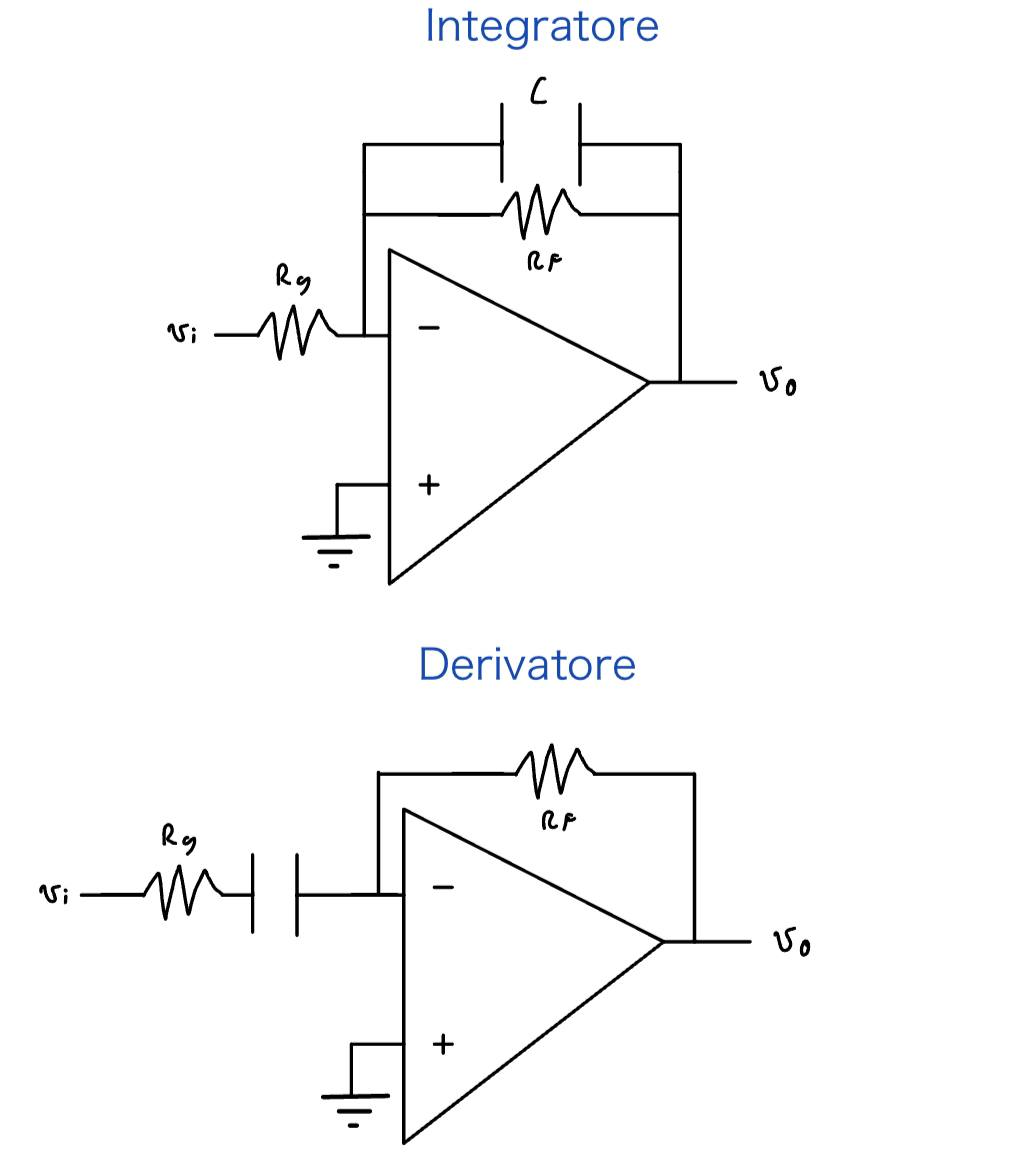
\includegraphics[scale=0.2]{schema.jpg}
\end{flushleft}
\section{Materiale e Strumenti}
\begin{multicols}{2}
    \begin{itemize}
    \item Fili di collegamento
    \item Breadboard
    \item Resistenza da $2.2k\Omega$
    \item Resistenza da $22k\Omega$
    \item Condensatore 4.7$\mu n$
    \item Amplificatore operazionale \textit{U741}
    \end{itemize}
    \vfill\null
    \columnbreak
    \begin{itemize}
    \item Multimetro
    \item Generatore di funzione
    \item Oscilloscopio
    \item Alimentazione DC 
    \end{itemize}
    \vfill\null
    \end{multicols}
\section{Contenuti Teorici}
Avendo come dati $R_F$,$R_G$ e C si può ricavare la frequenza di taglio con la formula $f_t=\frac{1}{2 \pi R_F C}$.\\
Se si divide questa frequenza per 10 si può notare con l’oscilloscopio che il circuito integratore lavora come aplificatore invertente, invece se si moltiplica per 10 sarà semplicemente un integratore.\\
Questo succede perchè a basse frequenze il condensatore diventa un circuito aperto poichè il condensatore va in 
saturazione.\\
Il contrario avviene con il derivatore, a basse frequenze fuonzionerà normalmente mentre ad alte frequenze
diventerà un amplificatore invertente poichè il condensatore sarà equivalente a un corto circuito.\\
Con la configurazione a derivatore da un'onda triangolare si aspetta un'onda quadra della quale calcoleremo l'ampiezza e il valore massimo.\\
Con la configurazione integratore invece ci si aspetta da un onda quadra un onda triangolare della quale andremo a misurare e calcolare la pendenza.\\
\subsection{Descrizione della Prova}
Dopo aver svolto i calcoli teorici vanno misurate le resistenze e verificato che il valore sia comparabile
a quello riportato tramite codice colore.\\
Dopodiche viene montato il circuito sulla Breadboard segendo lo schema e si regolano le tensioni di 
alimentazione Vcc+ e Vcc- per l’integrato.\\
Con l’ausilio dell’oscilloscopio si visualizza l’andamento della tensione di ingresso e di uscita per 
confrontarle e prendere i dati sperimentali.\\
Le misure con il derivatore verranno prese a $f=\frac{f_c}{10}$ mentre con l'integratore verranno prese due misure, una a $f=\frac{f_c}{10}$ e un'altra a $f=f_c \cdot 10$
\subsection{Oscilloscopio}
Configurazione Integratore:
\begin{figure}[h]
    \centering
   \includegraphics[scale=0.055]{integratore-altaf.jpg}
    \caption{integratore $f_c \cdot 10$}
\end{figure}
\begin{figure}[h]
    \centering
    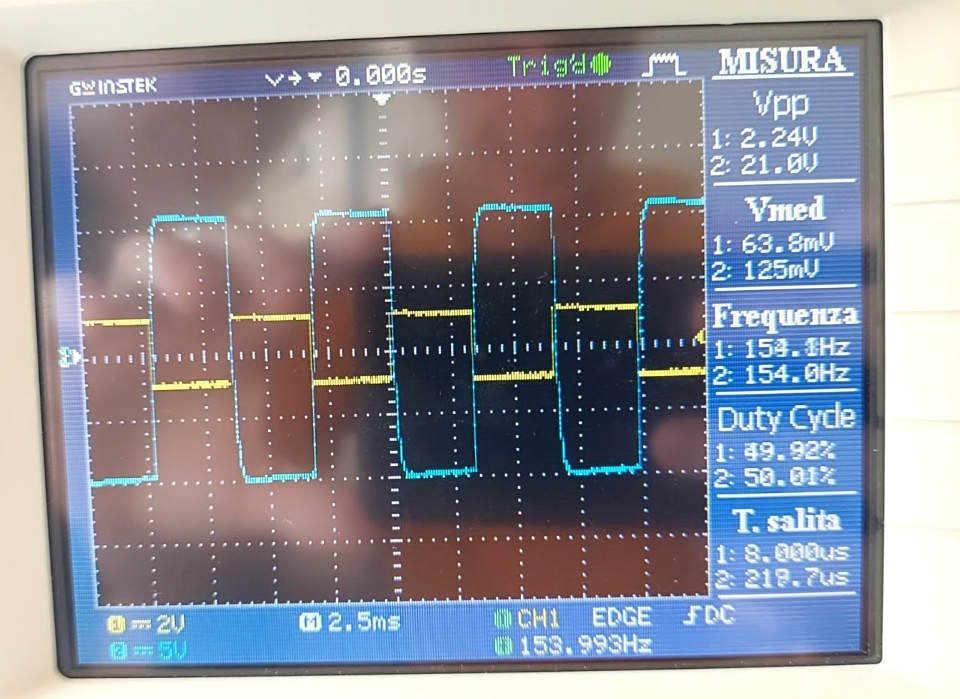
\includegraphics[scale=0.2]{integratore-bassaf.jpg}
    \caption{integratore $\frac{f_c}{10}$}
\end{figure}
\\
Configurazione Derivatore:
\begin{figure}[!h]
    \centering
    \includegraphics[scale=0.05]{derivatore.jpg}
    \caption{Derivatore $\frac{f_c}{10}$}

\end{figure}
\\

\subsection{Tabella}
Valore misurato resistenze:\\
\begin{center}
        \begin{tabular}{|p{2cm}|p{2cm}|}
            \hline
            \rowcolor{RoyalBlue} $R_F$ & $R_G$ \\
            \hline
            \rowcolor{CornflowerBlue} $21k\Omega$ & $2,14k\Omega$  \\ 
            \hline
        \end{tabular}
        \label{Valore resistenze}
\end{center}
\noindent
Configurazione integratore:\\
\begin{center}
    \begin{tabular}{|p{2cm} |p{2cm}|p{2cm} |p{2cm}|p{2cm} |p{2cm}|}
        \hline
        \rowcolor{RoyalBlue} $X1(V)$ & $X2(V)$& $\Delta (X)$ & $Y1(us)$ & $Y2(us)$ & $\Delta Y(us)$   \\
        \hline
        \rowcolor{CornflowerBlue} $1,6$ & $-1,4$ & $3$ & $1$ & $33$  & $32$\\ 
        \hline
    \end{tabular}
\end{center}

\noindent Configurazione derivatore :\\
\begin{center}
    \begin{tabular}{|p{2cm} |p{2cm}|}
        \hline
        \rowcolor{RoyalBlue} $v_i$ & $v_o$  \\
        \hline
        \rowcolor{CornflowerBlue} $1V$ & $1.32V$  \\ 
        \hline
    \end{tabular}
    \label{Valore resistenze}
\end{center}

\subsection{Commento dei dati raccolti in tabella}

\section{Elaborazione dei dati raccolti}
\subsection{Calcoli}
Configurazione integratore:\\
$f_c=\frac{1}{2 \pi R_F C}=\frac{1}{2 \pi 22 k\Omega 4.7\mu n }=1.54KHz$\\
\\
\textit{Pendenza}=$-\frac{1}{R_G}=-\frac{1}{2,2k\Omega \cdot 4,7 \mu n}=-96711 $\\
\\
\textit{Pendenza}=$\frac{\Delta Y}{\Delta X}=\frac{1.6-(-1.4)}{(1\cdot 10^{-6})-(33\cdot 10^{-6})}$=-93750\\
\\
Discrepanza=$\frac{Val. sperimentale}{Val. calcolato}=\frac{-96711}{-93750}=1.03$\\
\\
\\
Configurazione derivatore:\\
$f_c=\frac{1}{2 \pi R_G C}=\frac{1}{2 \pi 2,14 k\Omega 4.7\mu n }=15.4KHz$\\
%\\
%$v_o=-R_G \cdot C=-2,22k\Omega \cdot 4,7 \mu n=1.03V$\\
\section{Analisi critica dei risultati e conclusioni}
I valori sperimentali coincidono con quelli  oteniti dai calcoli apparte una discrepanza comunque accettabile
tra i due valori di pendenza della retta.\\
\end{document}